\section{Board Configuration}\label{sec:BoardConfiguration}

This section introduces the model for the board configuration, which allows users to control the resources required to display a board within the prototype (e.g., board and card component resources). The board configuration is part of the \textit{DataManager}, which is eccenca’s front-end allowing users to author and explore semantic content.

\subsection{Config Definition}

The graph-based board configuration is defined by different terms, primarily \tracknshrink{RDF(S)}, \acrshort*{OWL}, and \acrshort*{SHACL}. However, this subsection only highlights key aspects in prefixed Turtle notation; the entire graph can be found in the appendix of this work. Fundamentally, the \acrshort*{RMB} is defined as an \acrshort{owl}\texttt{Ontology} and the board configuration as an \acrshort{owl}\texttt{Class}, as defined in \autoref{lst:BoardConfigGlobal}.

\begin{spacing}{0.9}
    \lstset{language=N3,escapechar=|}
    \begin{lstlisting}[
    label={lst:BoardConfigGlobal},
    xleftmargin=19em, % this needs to be manually adjusted to center the frame
    xrightmargin=-23em, % this needs to be manually adjusted to center the frame
    caption={[\tracknshrink{RMB} \& Board Configuration in Turtle]Exemplary sample of the \acrshort*{RMB} and the board configuration as an \acrshort*{OWL} ontology and class.}]
|\acrshort{rmb}|
  a |\acrshort{owl}|Ontology ;
  |\acrshort{rdfs}|label "Resource Management Board" .
|\acrshort{rmb}|BoardConfig
  a |\acrshort{owl}|Class ;
  |\acrshort{rdfs}|label "Board Configuration" .
\end{lstlisting}
\end{spacing}

\noindent As requested by the first functional requirement (\tracknshrink{FR}\textsubscript{1}), the board configuration contains various properties to describe a board. \autoref{lst:BoardComponentResources} illustrates the definition of the board component resources.


\begin{spacing}{0.9}
    \lstset{language=N3,escapechar=|}
    \begin{lstlisting}[
    label={lst:BoardComponentResources},
    xleftmargin=21em, % this needs to be manually adjusted to center the frame
    xrightmargin=-17em, % this needs to be manually adjusted to center the frame
    caption={[Board Component Resources in Turtle]Exemplary sample of the definition for the board component resources.}]
|\acrshort{rmb}|cardsClass
  a |\acrshort{owl}|ObjectProperty ;
  |\acrshort{rdfs}|label "Cards Class(es)" ;
  |\acrshort{rdfs}|domain |\acrshort{rmb}|BoardConfig .
  
|\acrshort{rmb}|cardsColumnProperty
  a |\acrshort{owl}|ObjectProperty ;
  |\acrshort{rdfs}|label "Column Property" ;
  |\acrshort{rdfs}|domain |\acrshort{rmb}|BoardConfig .
  
|\acrshort{rmb}|cardsLaneProperty
  a |\acrshort{owl}|ObjectProperty ;
  |\acrshort{rdfs}|label "Lane Property" ;
  |\acrshort{rdfs}|domain |\acrshort{rmb}|BoardConfig .
\end{lstlisting}
\end{spacing}


\noindent \acrshort*{SHACL} is used to validate the graph by certain conditions. Moreover, eccenca’s \textit{DataManager} relies on these shapes to render their front-end \acrshort*{UI}. \autoref{lst:CardsClassSHACL} illustrates the use of \acrshort*{SHACL} to specify the \texttt{cardsClass} property further. For example, the property \acrshort{sh}\texttt{nodeKind} (line 4) has a value of \acrshort{sh}\texttt{IRI}. This constraint means that nodes confirming to \acrshort{rmb}\texttt{cardsClass} must be of type \acrshort*{IRI}. Moreover, it can be observed that \acrshort{sh}\texttt{minCount} (line 6) is defined, while \acrshort{sh}\texttt{maxCount} is not. This is on purpose since cards are allowed to refer to multiple classes (or resources). In contrast, the shape specifications for column and lane properties would contain both conditions, since a \acrshort{sh}\texttt{minCount} of \texttt{1} defines a property as mandatory, whereas \acrshort{sh}\texttt{maxCount} defines a maximum number of allowed instances.


\begin{spacing}{0.9}
    \lstset{language=N3,escapechar=|}
    \begin{lstlisting}[
    label={lst:CardsClassSHACL},
    xleftmargin=21em, % this needs to be manually adjusted to center the frame
    xrightmargin=-17em, % this needs to be manually adjusted to center the frame
    caption={[Example of a \tracknshrink{SHACL} Definition]Sample \tracknshrink{SHACL} specification for the property \texttt{cardsClass}.}]
|\acrshort{rmb}|cardsClassSHACL
  a |\acrshort{sh}|PropertyShape ;
  |\acrshort{sh}|class |\acrshort{owl}|Class ;
  |\acrshort{sh}|nodeKind |\acrshort{sh}|IRI ;
  |\acrshort{sh}|path |\acrshort{rmb}|cardsClass ;
  |\acrshort{sh}|minCount 1 .
\end{lstlisting}
\end{spacing}

\vspace*{-1.40em}

\subsection{Config Properties and Relations}

The board configuration consists of ten properties, as requested by the first functional requirement (\tracknshrink{FR}\textsubscript{1} on page \pageref{FR1}). \autoref{tab:BoardConfig} provides a more specific overview of all properties as defined by the graph for board configuration. Note that the last column, \tracknshrink{RMB} Defaults, is referring to default values being used by the \tracknshrink{RMB}, as requested by \tracknshrink{FR}\textsubscript{2}.



\begin{table}[H]\centering%\small
\libertineLF
\resizebox{\textwidth}{!}{%
\begin{tabular}{lll} 
	\toprule
	Board Config Object \textrightarrow{} \acrshort{sh}\texttt{nodeKind} & Object Description & \textit{required}/\tracknshrink{RMB Default}\\ 
	\midrule
	\multicolumn{3}{l}{General Board Properties}\\
	\cmidrule(rl){1-3}
	\acrshort{rdfs}\texttt{label} \textrightarrow{} \acrshort{sh}\texttt{Literal} & The name of the board & \textit{required} \\
	\acrshort{dct}\texttt{description} \textrightarrow{} \acrshort{sh}\texttt{Literal} & Descriptive text about the board’s intention & \texttt{""} \\
	\acrshort{rmb}\texttt{cardsGraph} \textrightarrow{} \acrshort{sh}\texttt{IRI} & Graph, which is used to get the cards from & \textit{required} \\
	\acrshort{rmb}\texttt{boardLimit} \textrightarrow{} \acrshort{sh}\texttt{Literal} & Integer to set the card display limit on a board & 100 \\ \cmidrule(rl){1-3}
	\multicolumn{3}{l}{Board Component Resources}\\
	\cmidrule(rl){1-3}
	\acrshort{rmb}\texttt{cardsClass} \textrightarrow{} \acrshort{sh}\texttt{IRI} & Card resources (multiple) & \textit{required} \\
	\acrshort{rmb}\texttt{cardsColumnProperty} \textrightarrow{} \acrshort{sh}\texttt{IRI} & Column resource (mutation property)  & \textit{required} \\
	\acrshort{rmb}\texttt{cardsLaneProperty} \textrightarrow{} \acrshort{sh}\texttt{IRI} & Swimlane resource & \texttt{""} \\
	\cmidrule(rl){1-3}
	\multicolumn{3}{l}{Card Component Resources}\\
	\cmidrule(rl){1-3}
	\acrshort{rmb}\texttt{cardsDescriptionProperty} \textrightarrow{} \acrshort{sh}\texttt{IRI} & The property to fill the card body & \acrshort{dct}\texttt{description} \\
	\acrshort{rmb}\texttt{cardsAdditionalFieldProperty} \textrightarrow{} \acrshort{sh}\texttt{IRI} & Resources referring to additional properties & \texttt{""} \\
	\acrshort{rmb}\texttt{cardsModifiedProperty} \textrightarrow{} \acrshort{sh}\texttt{IRI} & Property used to save modified timestamps & \acrshort{dct}\texttt{modified} \\
\end{tabular}}
	\caption[Board Configuration Properties]{Board Configuration Properties.}
	\label{tab:BoardConfig}
	\libertineOsF
\end{table}





\noindent To illustrate the structure, relations, and cardinalities of the board configuration, the class diagram in \autoref{fig:BoardConfigUML} highlights the class for the board configuration along with its properties. To transfer existing conventions from the traditional \tracknshrink{UML} class diagram to the domain of \acrshort*{RDF}, the work by Tong and colleagues (\citeyear{Tong2015}) is used as a reference. \citeauthor{Tong2015} propose a model that allows a \textit{“Construction of \tracknshrink{RDF(S)} from \tracknshrink{UML} Class Diagrams.”} Although they neither included \acrshort*{OWL} nor \acrshort*{SHACL} in their model, it is a helpful guide that is applicable in both directions. For example, they provided two tables that map the main elements and datatypes of \tracknshrink{UML} to \tracknshrink{RDF(S)} and vice versa \parencite[241,243]{Tong2015}.

Nevertheless, in the following, the most important key aspects for mapping the board configuration to a \tracknshrink{UML} class diagram are outlined. Furthermore, based on their publication, the corresponding transformation rule and page will be used: First and foremost, \acrshort*{RDF} classes are mapped to regular \tracknshrink{UML} classes (Rule 2, p.~241). This rule applies to the board configuration since it is defined as an \acrshort{owl}\texttt{Class} (see \autoref{lst:BoardConfigGlobal}). \acrshort*{RDF} properties whose values are literals (i.e., specified by an xsd datatype) become \tracknshrink{UML} class attributes (Rule 4, p.~241), as exemplarily depicted by the \acrshort{rdfs}\texttt{label} within classes. Lastly, properties whose values are resources, and their \acrshort{rdfs}\texttt{domain} refers to their parent class become an \tracknshrink{UML} aggregation (Table 1, p. 241 and Rule 6, p. 242).

Since \citeauthor{Tong2015} did not incorporate \acrshort*{OWL} and \acrshort*{SHACL}, they concluded that cardinality could not be expressed in their model (p. 244). However, both \acrshort*{OWL} and \acrshort*{SHACL} allow to define cardinalities. Specifically, \acrshort*{OWL} has a dedicated property (i.e., \acrshort{owl}\texttt{minCardinality} and \acrshort{owl}\texttt{maxCardinality}), whereas \acrshort*{SHACL} uses the previous mentioned \acrshort{sh}\texttt{minCount} and \acrshort{sh}\texttt{maxCount} properties which may also be used to describe cardinality. \autoref{fig:BoardConfigUML} depicts the corresponding cardinalities between each relation. For this prototypical configuration, \acrshort{rmb}\texttt{cardsClass} and \acrshort{rmb}\texttt{cardsAdditionalFieldProperty} are the only elements that allow multiple instances (as outlined in \tracknshrink{FR}\textsubscript{1} and \tracknshrink{FR}\textsubscript{17} resp.).





\begin{figure}[H]
\centering
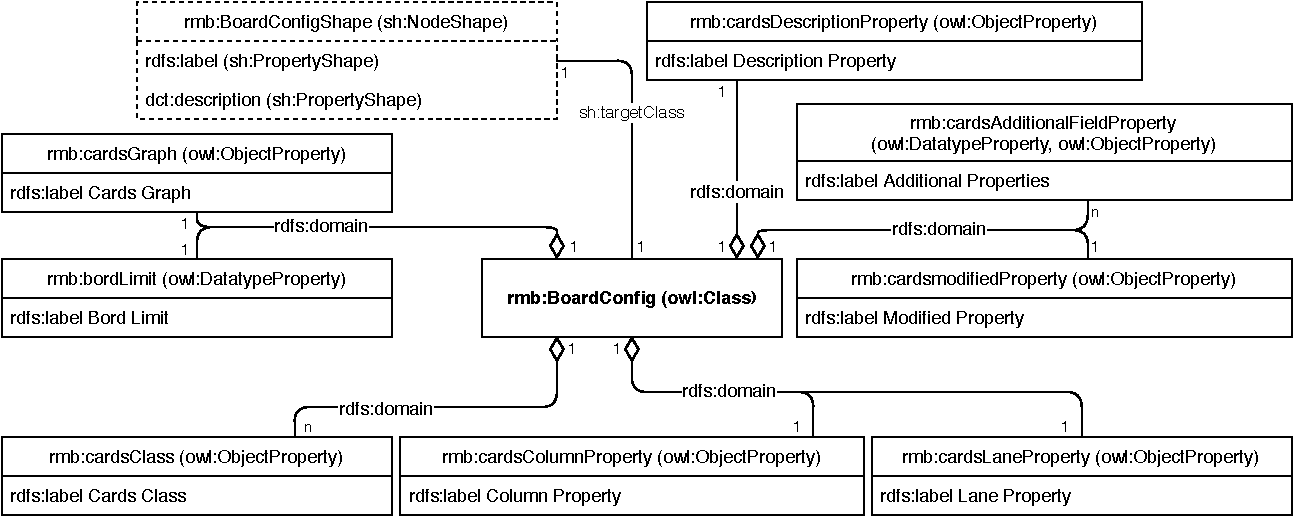
\includegraphics[width=\linewidth]{img/BoardConfigUML.pdf}
	\caption[Board Configuration Graph as \tracknshrink{UML} Class Diagram]{The prototypical board configuration graph represented as a \tracknshrink{UML} class diagram.}
	\label{fig:BoardConfigUML}
\end{figure}


\subsection{Config Instance \& Usage}


\noindent For demonstration purposes, \autoref{lst:FOAFBoardConfig} defines a particular instance of a board configuration with the data requested by the first use case (for reference see the board and card component resources on page \pageref{par:FOAF-BCR}). Note that neither developers nor users need to define a new board configuration in this manner; instead, users define a board using eccenca’s \textit{DataManger} which will generate a similar specification:

\begin{spacing}{0.9}
    \lstset{language=N3,escapechar=|}
    \begin{lstlisting}[
    label={lst:FOAFBoardConfig},
    xleftmargin=9em, % this needs to be manually adjusted to center the frame
    xrightmargin=-9em, % this needs to be manually adjusted to center the frame
    caption={[Example for an Instance of the Board Configuration]A board configuration instance of the first use case (\tracknshrink{FOAF} Term Status).}]
|\acrshort{rmb}|foaf-term-status
  a |\acrshort{rmb}|BoardConfig ;
  |\acrshort{rdfs}|label "FOAF Term Status" ;
  |\acrshort{dct}|description "Manages terms by their status in the FOAF namespace" ;
  |\acrshort{rmb}|cardsGraph |\acrshort{foaf}| ;
  |\acrshort{rmb}|cardsClass |\acrshort{owl}|Class, |\acrshort{owl}|DatatypeProperty, |\acrshort{owl}|ObjectProperty ;
  |\acrshort{rmb}|cardsColumnProperty |\acrshort{vs}|term_status ;
  |\acrshort{rmb}|cardsLaneProperty |\acrshort{rdf}|type ;
  |\acrshort{rmb}|cardsDescriptionProperty |\acrshort{rdfs}|comment .
\end{lstlisting}
\end{spacing}


\noindent The \textit{DataManager} relies on a graph that contains shape definitions to render its \acrshort*{UI}. In other words, a (compatible) graph gets translated to a user interface. When importing the entire board configuration graph (see appendix) into eccenca’s \textit{DataManager}, the front-end will render the graph as described in \autoref{fig:BoardConfigs}. While \autoref{fig:BoardConfigs} (A) illustrates the interface when defining a new board configuration, \autoref{fig:BoardConfigs} (B) shows the configuration for the first use case. After creating a new board configuration, as in (B), this particular instance will be added to the board configuration graph. In other words, exporting the board configuration graph of \autoref{fig:BoardConfigs} (B), would lead to a graph with similar data as \autoref{lst:FOAFBoardConfig}.

The properties listed in \autoref{fig:BoardConfigs} (A) correspond to all properties requested in the first functional requirement (see \tns{FR}\textsubscript{1}) or as specified in \autoref{tab:BoardConfig}. Moreover, as image (A) shows, there are four required fields: the board’s name, graph, card class(es), and column property. Thus, the \tns{UI} requires the user to add a resource. This \tns{UI} functionality is derived from a resource \acrshort{sh}\texttt{minCount} property set to value 1, making it mandatory to define a resource, as mentioned earlier.


\autoref{fig:BoardConfigs} (B) depicts the setup for the \textit{\acrshort*{FOAF} Term Status} use case (see page \pageref{par:FOAF-BCR} for the board and card component resources). The class(es) field contains multiple resources since a \acrshort{sh}\texttt{maxCount} is not defined for this property.


\begin{figure}[H]
    \libertineLF
	\centering \begin{tikzpicture}
	\node[anchor=south west,inner sep=0] (image) at (0,0,0) {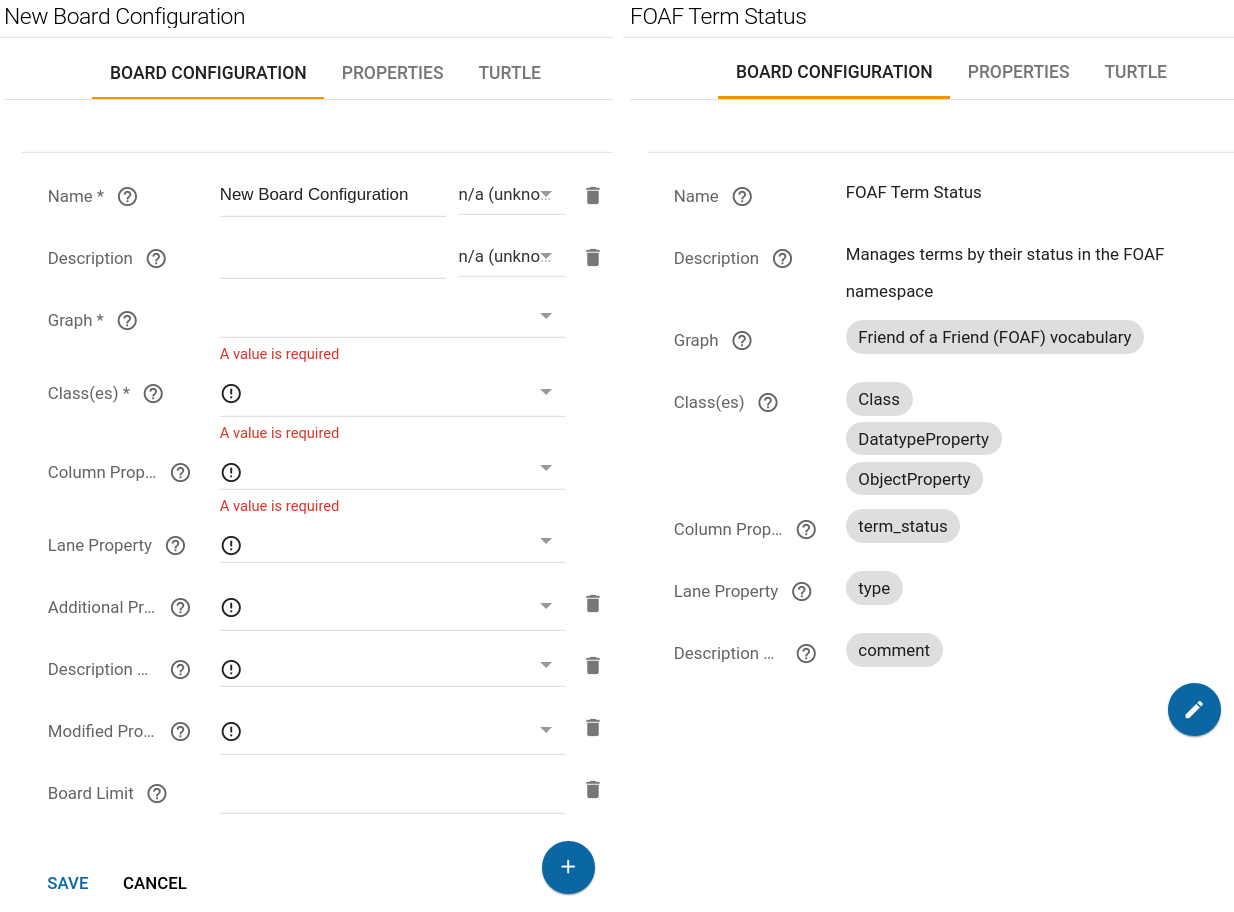
\includegraphics[width=\linewidth]{img/Board-Configurations.png}};
	\begin{scope}[x={(image.south east)},y={(image.north west)}]

	\draw (0.250,1.030) node[anchor=west] {(A)};
	\draw (0.740,1.030) node[anchor=west] {(B)};

	\end{scope}
	\end{tikzpicture}
	\caption[Board Configuration Graph in eccenca’s \textit{DataManager}]{Board configuration graph represented in eccenca’s \textit{DataManager}. (A) is showing all defined fields of the board configuration. (B) is showing an actual instance of a board configuration (i.e., the first use case).}
	\label{fig:BoardConfigs}
	\libertineOsF
\end{figure}


